\section{La sustentation et l'aile}

\subsection{Les axes}
\subsubsection{Les 4 forces}
\begin{figure}[H]
		\centering
  		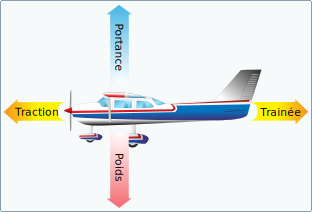
\includegraphics[width=0.8\textwidth]{04-Aerodynamique/img/forces.pdf}
  		\legende{Les 4 forces}{img:forces}	
\end{figure}

\subsection{L'aile}

\subsubsection{Description générale}
Toute aile est composée de plusieurs parties distinctes :
\begin{itemize}
	\item L'\gls{intrados} est la partie inférieure de l'aile. Lorsque l'aile se déplace dans une masse d'air, l'intrados est le siège d'une surpression.
	\item L'\gls{extrados} est la partie supérieure de l'aile. Lorsque l'aile se déplace dans une masse d'air, l'extrados est le siège d'une dépression (l'aile est aspirée vers le haut).
	\item Le \gls{bord d'attaque} \anglais{leading edge} est le point le plus en avant d'un profil d'aile. C'est à ce point que l'air entrera en contact en premier avec l'aile. Il s'agit généralement d'une surface  courbe.
	\item Le \gls{bord de fuite} \anglais{trailing edge} est le point le plus en arrière d'un profil d'aile.  Il s'agit généralement d'une pointe.
\end{itemize}

	\begin{figure}[H]
  	\centering
    \includegraphics[width=0.8\textwidth]{04-Aerodynamique/img/profilAile}
  	\legende{Profil d'une aile}{img:profilAile}
	\end{figure}	
	
	\astuce{Pour se souvenir ou sont situés l'intrados et l'extrados : quand l'avion vol à plat, l'extrados fait face à l'extérieur de la planète, l'intrados regarde vers l'intérieur de la planète.} 
	
\subsubsection{Répartition des pressions autour d'une aile}
	\begin{figure}[H]
		\centering
  		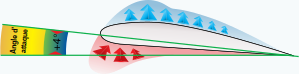
\includegraphics[width=0.8\textwidth]{04-Aerodynamique/img/pressionProfilSelonAngleAttaque4deg.pdf}
  		\legende{La pression autour d'une aile}{img:pressionProfilSelonAngleAttaque}
	\end{figure}	


\subsection{La portance}
\begin{figure}[H]
		\centering
  		\includegraphics[width=0.65\textwidth]{04-Aerodynamique/img/portanceTraineeFinesse_portance.pdf}
  		\legende{Portance en fonction de l'angle d'incidence de l'aile}{img:portanceTraineeFinesse}
	\end{figure}	

\subsubsection{Expression algébrique de la portance}
	\begin{center}
		\huge{$Z = \dfrac{1}{2}\rho S V^2 Cz$}
	\end{center}

\subsection{La trainée}
\begin{figure}[H]
		\centering
  		\includegraphics[width=0.65\textwidth]{04-Aerodynamique/img/portanceTraineeFinesse_trainee.pdf}
  		\legende{Trainée en fonction de l'angle d'incidence de l'aile}{img:portanceTraineeFinesse}
	\end{figure}	

\subsubsection{Expression algébrique de la trainée}
	\begin{center}
		\huge{$X = \dfrac{1}{2}\rho S V^2 Cx$}
	\end{center}
	
\subsection{Finesse}

\subsection{Polaire d'une aile}
Il est possible de tracer sur un graphique la portance (Cz) en fonction de la trainée (Cx).
\begin{figure}[H]
		\centering
  		\includegraphics[width=0.5\textwidth]{04-Aerodynamique/img/polaireAileMeilleureFinesse.pdf}
  		\legende{Polaire d'une aile, avec point de meilleure finesse}{img:polaireAileMeilleureFinesse}
\end{figure}	

Obtenue en traçant la portance $C_z$ en fonction de la trainée $C_x$. On peut identifier sur cette courbe plusieurs points caractéristiques :
 		\begin{itemize}
 			\item $A$ : $Cz = 0 \Rightarrow$ portance nulle
 			\item $B$ : trainée $C_x$ minimale
 			\item $C$ : $\dfrac{C_z}{C_x}$ minimum $\Rightarrow$ finesse maximale
 			\item $D$ : portance $C_z$ maximale
 			\item $E$ : décrochage
 		\end{itemize}

\subsection{Dispositifs hypersustentateurs et destructeurs de portance}
	\subsubsection{Dispositifs hypersustentateurs}
		\paragraph{Volets}
		\begin{figure}[H]
			\centering
  			\includegraphics[width=0.4\textwidth]{04-Aerodynamique/img/hypersustentateurs/voletsDeCourbure.pdf}
  			\legende{Volets de courbure}{img:voletsDeCourbure}	
		\end{figure}
		
		\begin{figure}[H]
			\centering
  			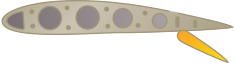
\includegraphics[width=0.4\textwidth]{04-Aerodynamique/img/hypersustentateurs/voletDIntrados.pdf}
  			\legende{Volets d'intrados}{img:voletDIntrados}	
		\end{figure}
		
		\begin{figure}[H]
			\centering
  			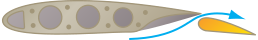
\includegraphics[width=0.4\textwidth]{04-Aerodynamique/img/hypersustentateurs/voletFowler.pdf}
  			\legende{Volets Fowler}{img:voletFowler}	
		\end{figure}
		
		\begin{figure}[H]
			\centering
  			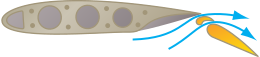
\includegraphics[width=0.4\textwidth]{04-Aerodynamique/img/hypersustentateurs/voletFowlerAFente.pdf}
  			\legende{Volets Fowler}{img:voletFowlerAFente}	
		\end{figure}
		
		\paragraph{Becs}
		\begin{figure}[H]
			\centering
  			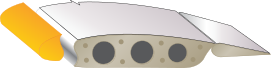
\includegraphics[width=0.4\textwidth]{04-Aerodynamique/img/hypersustentateurs/becs.pdf}
  			\legende{Bacs de bord d'attaque}{img:becs}	
		\end{figure}
		
	\subsubsection{Dispositifs destructeurs de portance}
	